\documentclass{beamer}

\usepackage[utf8]{inputenc}
\usepackage[francais]{babel}
\usepackage{tikz}

% FAMFAMFAM.com colors
\definecolor{mpink}{RGB}{255,11,91}
\definecolor{mblue}{RGB}{11,206,255}
\definecolor{mgreen}{RGB}{123,255,45}

\usetheme{Warsaw}

\setbeamertemplate{navigation symbols}{}
\setbeamertemplate{footline}[frame number]

\definecolor{Backdrop}{RGB}{85, 98, 112}
\definecolor{Foreground}{RGB}{238, 238, 238}
\definecolor{Fabulous}{RGB}{210, 111, 127}

\usecolortheme[named=Backdrop]{structure}
\setbeamerfont{title}{series=\bfseries}
\setbeamercolor{title}{bg=Backdrop}
\setbeamercolor{frametitle}{fg=white, bg=Backdrop}
\setbeamercolor{normal text}{fg=Backdrop, bg=white}
\setbeamerfont{alerted text}{series=\bfseries}
\setbeamercolor{alerted text}{fg=Backdrop!120}
\setbeamertemplate{blocks}[rounded][shadow=true]
\setbeamerfont{block title}{series=\bfseries}
\setbeamercolor{block title}{fg=white, bg=Backdrop!105}
\setbeamercolor{block body}{fg=Foreground, bg=Backdrop!80}
\setbeamertemplate{items}[circle]
\setbeamercolor{item}{fg=Fabulous!50}
\setbeamerfont{footline}{size=\small}

\title{Recherche décentralisée de connexité pour réseaux de capteurs mobiles}
\author{Merwan Achibet}
\institute{Université du Havre}
\date{Jeudi 16 février 2012}

\AtBeginSection[]{
  \begin{frame}{Sommaire}
  \small \tableofcontents[currentsection, hideothersubsections]
  \end{frame}
}

\begin{document}

\maketitle

\section{Introduction}

\begin{frame}

  \begin{block}{Problème}
    \begin{itemize}
    \item{Des capteurs sont lâchés dans un espace}
    \item{Doivent être proches pour communiquer}
    \item{Sont mobiles}
    \item{Sont vulnérables aux pannes}
    \item{$\rightarrow$ Un réseau dynamique}
    \end{itemize}
  \end{block}

  \vfill

  Deux questions :
  \begin{enumerate}
  \item{Comment savoir si le réseau est connexe ?}
  \item{Comment rendre le réseau connexe ?}
  \end{enumerate}

  \vfill

  \alert{Et ce, de manière décentralisée !}

\end{frame}

\newcommand{\tikzbullet}[1]{
  \begin{tikzpicture}
    \draw[fill=#1,#1] (0,0) circle (0.1);
  \end{tikzpicture}
}

\begin{frame}

  \begin{figure}
    \begin{tikzpicture}

  \draw (0,0) -- (-1,1);

  \drawSensor{0}{0}{2}{red}
  \drawSensor{-1}{1}{2}{blue}
  \drawSensor{2.5}{1}{2}{green}

\end{tikzpicture}

  \end{figure}

  \vfill

  \begin{itemize}
  \item[$\blacktriangleright$]{\tikzbullet{mpink} et \tikzbullet{mblue} sont connectés}
  \item[$\blacktriangleright$]{\tikzbullet{mgreen} est isolé}
  \end{itemize}

\end{frame}

\section{Déterminer la connexité}

\begin{frame}

  \begin{block}{Cadre}
    \begin{itemize}
      \item{On se place du point de vue d'un capteur $c$}
      \item{On considère que le réseau est connexe si $c$ pense que le réseau
        est connexe}
    \end{itemize}
  \end{block}

  \vfill

  \begin{block}{}
    \begin{itemize}
      \item{Peut être ramené à un problème de comptage décentralisé}
      \item{Les capteurs connaissent $n$}
      \item{Un capteur sait que $\tilde{n}$ n\oe uds sont sur sa
        composante connexe}
      \item{Si $\tilde{n} = n$, le réseau est connexe}
    \end{itemize}
  \end{block}

\end{frame}


\begin{frame}

  \frametitle{Deux niveaux de certitude}

  \begin{block}{Dans le voisinage}
    \begin{itemize}
    \item{On est certain de l'arrivée d'un nouveau voisin}
    \item{On peut surveiller le départ des voisins}
    \end{itemize}
  \end{block}

  \vfill

  \begin{block}{Au loin}
    \begin{itemize}
    \item{Aucune certitude}
    \end{itemize}
  \end{block}

  \vfill

  Idée :
  \begin{itemize}
  \item{Un capteur partage régulièrement sa vision du réseau}
  \item{Chaque information de présence (ou d'absence) est datée}
  \item{On intègre la vision des autres capteurs sous conditions}
  \end{itemize}

\end{frame}

\begin{frame}

  \frametitle{Dans la mémoire interne de chaque capteur}

  \begin{block}{N}
    Contient les voisins de $c$.
  \end{block}

  \vfill

  Exemple : $\{b, f, z\}$
\end{frame}

\begin{frame}

  \frametitle{Dans la mémoire interne de chaque capteur}

  \begin{block}{C}
    Contient les n\oe uds que $c$ pensent connectés au réseau. Ses
    entrées sont des triplets $(x,t,s)$ avec
    \begin{itemize}
      \item{$x$ le n\oe ud dont l'on suppose la présence}
      \item{$t$ le temps de sa dernière détection}
      \item{$s$ le n\oe ud ayant transmis l'information (un voisin)}
    \end{itemize}
  \end{block}

  \vfill

  Exemple : $\{(a,23,c),(f,5,a)\}$

\end{frame}

\begin{frame}

  \frametitle{Dans la mémoire interne de chaque capteur}

  \begin{block}{D}
    Contient les n\oe uds dont $c$ doute de l'appartenance au
    réseau. Ses entrées sont des paires $(x,t)$ avec
    \begin{itemize}
      \item{$x$ le n\oe ud dont l'on suppose l'absence}
      \item{$t$ le temps auquel son absence a été détectée}
    \end{itemize}
  \end{block}

  \vfill

  Exemple : $\{(p,103)\}$

\end{frame}

\begin{frame}

  \frametitle{Modification par ses propres observations}

  \begin{block}{$c$ reçoit un message d'un nouveau voisin $c'$}
    $c' \rightarrow$ N, C
  \end{block}

  \vfill

  \begin{block}{Pas de message d'un voisin $c'$ enregistré depuis un
      certain temps (surveillance)}
    $N, C \rightarrow$ D
  \end{block}

\end{frame}

\begin{frame}

  \frametitle{Modification par évaluation des rumeurs}

  \`A chaque réception d'un message, on l'évalue par rapport à nos
  connaissance pour juger quelles informations intégrer et quelles
  informations ignorer.

  \vfill

  \begin{block}{Critère d'évaluation}
    L'étiquette temporelle
  \end{block}

\end{frame}

\begin{frame}

  \frametitle{Quelques exemples}

  \begin{block}{$C'=\{\dots,(a,42,e)\}$ et aucune mention de $a$ dans C ou
    D}
      $\rightarrow C = \{\dots,(a,42,c')\}$
  \end{block}

  \vfill

  \begin{block}{$C'=\{\dots,(a,42,e)\}$ et $C=\{\dots,(a,28,f)\}$}
      $\rightarrow C = \{\dots,(a,42,c')\}$
  \end{block}

\end{frame}

\begin{frame}

  \frametitle{Quelques exemples}

  \begin{block}{$C'=\{\dots,(a,42,e)\}$ et $D=\{\dots(a,78,f)\}$}
      On ignore l'information
  \end{block}

  \vfill

  \begin{block}{$D'=\{\dots,(a,42,e)\}$ et $C=\{\dots,(a,28,f)\}$}
    $C = \{\dots\}$\\
    $D = \{\dots,(a,42,c')\}$
  \end{block}

\end{frame}

\begin{frame}

  \frametitle{\`A quoi sert la source ?}

  \begin{block}{$D'=\{\dots,(b,54,z)\}$ et
      $C=\{\dots,(a,23,b),(b,11,c)\}$}
    $(b,11,c)$ passe de C à D\\
    $(a,23,b)$ aussi car $b$ en est la source
  \end{block}

\end{frame}

\begin{frame}
  \begin{figure}
    \centering
    \begin{tikzpicture}

  \draw (180:2) node[draw,circle,fill=white] (a) {A};
\draw (270:1) node[draw,circle,fill=white] (d) {D};
\draw (0:2) node[draw,circle,fill=white] (c) {C};
\draw (90:1) node[draw,circle,fill=white] (b) {B};


  \draw (0,1.8) node {$D = \{\}$}
  ++(0,0.5) node {$C = \{\}$}
  ++(0,0.5) node {$N = \{\}$};

  \draw (2.3,0.7) node {$D = \{\}$}
  ++(0,0.5) node {$C = \{\}$}
  ++(0,0.5) node {$N = \{\}$};

  \draw (0,-2.8) node {$D = \{\}$}
  ++(0,0.5) node {$C = \{\}$}
  ++(0,0.5) node {$N = \{\}$};

  \draw (-2.3,0.7) node {$D = \{\}$}
  ++(0,0.5) node {$C = \{\}$}
  ++(0,0.5) node {$N = \{\}$};

\end{tikzpicture}

  \end{figure}
\end{frame}

\begin{frame}
  \begin{figure}
    \centering
    \begin{tikzpicture}

  \draw (180:2) node[draw,circle,fill=white] (a) {A};
\draw (270:1) node[draw,circle,fill=white] (d) {D};
\draw (0:2) node[draw,circle,fill=white] (c) {C};
\draw (90:1) node[draw,circle,fill=white] (b) {B};


  \draw[thick] (b) -- (c);
  \draw[thick] (c) -- (d);

  \draw (0,1.8) node {$D = \{\}$}
  ++(0,0.5) node {$C = \{(C,3)\}$}
  ++(0,0.5) node {$N = \{C\}$};

  \draw (2.3,0.7) node {$\{\}$}
  ++(0,0.5) node {$\{(C,3)\}$}
  ++(0,0.5) node {$\{C\}$};

  \draw (0,-2.8) node {$\{\}$}
  ++(0,0.5) node {$\{(C,3)\}$}
  ++(0,0.5) node {$\{C\}$};

  \draw (-2.3,0.7) node {$\{\}$}
  ++(0,0.5) node {$\{(C,3)\}$}
  ++(0,0.5) node {$\{C\}$};

\end{tikzpicture}

  \end{figure}
\end{frame}

\begin{frame}
  \begin{figure}
    \centering
    \begin{tikzpicture}

  \draw[fill=red,draw=none] (180:2) circle (0.45cm);

  \draw (180:2) node[draw,circle,fill=white] (a) {A};
\draw (270:1) node[draw,circle,fill=white] (d) {D};
\draw (0:2) node[draw,circle,fill=white] (c) {C};
\draw (90:1) node[draw,circle,fill=white] (b) {B};


  \draw[thick] (b) -- (c);
  \draw[thick] (c) -- (d);
  \draw[thick] (a) -- (b);

  \draw (0,1.8) node {$\{\}$}
  ++(0,0.5) node {$\{(C,1,C),\textcolor{red}{(A,2,A)}\}$}
  ++(0,0.5) node {$\{C,\textcolor{red}{A}\}$};

  \draw (2.3,0.7) node {$\{\}$}
  ++(0,0.5) node {$\{\}$}
  ++(0,0.5) node {$\{\}$};

  \draw (0,-2.8) node {$\{\}$}
  ++(0,0.5) node {$\{(C,1,C)\}$}
  ++(0,0.5) node {$\{C\}$};

  \draw (-2.3,0.7) node {$\{\}$}
  ++(0,0.5) node {$\{\}$}
  ++(0,0.5) node {$\{\}$};

\end{tikzpicture}

  \end{figure}
\end{frame}

\begin{frame}
  \begin{figure}
    \centering
    \begin{tikzpicture}

  \draw (180:2) node[draw,circle,fill=white] (a) {A};
\draw (270:1) node[draw,circle,fill=white] (d) {D};
\draw (0:2) node[draw,circle,fill=white] (c) {C};
\draw (90:1) node[draw,circle,fill=white] (b) {B};


  \draw[thick] (b) -- (c);
  \draw[thick] (c) -- (d);
  \draw[thick] (a) -- (b);

  \draw (0,1.8) node {$\{\}$}
  ++(0,0.5) node {$\{(C,1,C),(A,2,A)\}$}
  ++(0,0.5) node {$\{C,A\}$};

  \draw (2.3,0.7) node {$\{\}$}
  ++(0,0.5) node {$\{(B,3,B),(A,2,B))\}$}
  ++(0,0.5) node {$\{B\}$};

  \draw (0,-2.8) node {$\{\}$}
  ++(0,0.5) node {$\{(C,1,C)\}$}
  ++(0,0.5) node {$\{C\}$};

  \draw (-2.3,0.7) node {$\{\}$}
  ++(0,0.5) node {$\{(B,3,B),(C,1,B)\}$}
  ++(0,0.5) node {$\{B,C\}$};

\end{tikzpicture}

  \end{figure}
\end{frame}

\begin{frame}
  \begin{figure}
    \centering
    \begin{tikzpicture}

  \draw[fill=red,draw=none] (180:2) circle (0.45cm);

  \draw (180:2) node[draw,circle,fill=white] (a) {A};
\draw (270:1) node[draw,circle,fill=white] (d) {D};
\draw (0:2) node[draw,circle,fill=white] (c) {C};
\draw (90:1) node[draw,circle,fill=white] (b) {B};


  \draw[thick] (b) -- (c);
  \draw[thick] (c) -- (d);
  \draw[thick] (a) -- (b);
  \draw[thick] (a) -- (d);

  \draw (0,1.8) node {$\{\}$}
  ++(0,0.5) node {$\{(C,1,C),(A,4,A)\}$}
  ++(0,0.5) node {$\{C,A\}$};

  \draw (2.3,0.7) node {$\{\}$}
  ++(0,0.5) node {$\{(B,3,B),(A,2,B))\}$}
  ++(0,0.5) node {$\{B\}$};

  \draw (0,-2.8) node {$\{\}$}
  ++(0,0.5) node {$\{(C,1,C),(A,4,A),(B,3,A))\}$}
  ++(0,0.5) node {$\{C,A\}$};

  \draw (-2.3,0.7) node {$\{\}$}
  ++(0,0.5) node {$\{(B,3,B),(C,1,B)\}$}
  ++(0,0.5) node {$\{B,C\}$};

\end{tikzpicture}

  \end{figure}
\end{frame}

\begin{frame}
  \begin{figure}
    \centering
    \begin{tikzpicture}

  \draw (180:2) node[draw,circle,fill=white] (a) {A};
\draw (270:1) node[draw,circle,fill=white] (d) {D};
\draw (0:2) node[draw,circle,fill=white] (c) {C};
\draw (90:1) node[draw,circle,fill=white] (b) {B};


  \draw[thick] (c) -- (d);
  \draw[thick] (a) -- (d);

  \draw (0,1.8) node {$\{\}$}
  ++(0,0.5) node {$\{(C,1,C),(A,4,A)\}$}
  ++(0,0.5) node {$\{C,A\}$};

  \draw (2.3,0.7) node {$\{(B,10),(A,10)\}$}
  ++(0,0.5) node {$\{\}$}
  ++(0,0.5) node {$\{\}$};

  \draw (0,-2.8) node {$\{\}$}
  ++(0,0.5) node {$\{(C,1,C),(A,4,A),(B,3,A))\}$}
  ++(0,0.5) node {$\{C,A\}$};

  \draw (-2.3,0.7) node {$\{\}$}
  ++(0,0.5) node {$\{(B,3,B),(C,1,B)\}$}
  ++(0,0.5) node {$\{B,C\}$};

\end{tikzpicture}

  \end{figure}
\end{frame}

\begin{frame}
  \begin{figure}
    \centering
    \begin{tikzpicture}

  \draw (180:2) node[draw,circle,fill=white] (a) {A};
\draw (270:1) node[draw,circle,fill=white] (d) {D};
\draw (0:2) node[draw,circle,fill=white] (c) {C};
\draw (90:1) node[draw,circle,fill=white] (b) {B};


  \draw[thick] (c) -- (d);
  \draw[thick] (a) -- (d);

  \draw (0,1.8) node {$\{\}$}
  ++(0,0.5) node {$\{(C,1,C),(A,4,A)\}$}
  ++(0,0.5) node {$\{C,A\}$};

  \draw (2.3,0.7) node {$\{(B,10),(A,10)\}$}
  ++(0,0.5) node {$\{\}$}
  ++(0,0.5) node {$\{\}$};

  \draw (0,-2.8) node {$\{\}$}
  ++(0,0.5) node {$\{(C,1,C),(A,11,A),(B,3,A))\}$}
  ++(0,0.5) node {$\{C,A\}$};

  \draw (-2.3,0.7) node {$\{\}$}
  ++(0,0.5) node {$\{(B,3,B),(C,1,B)\}$}
  ++(0,0.5) node {$\{B,C\}$};

\end{tikzpicture}

  \end{figure}
\end{frame}

\begin{frame}
  \begin{figure}
    \centering
    \begin{tikzpicture}

  \draw (180:2) node[draw,circle,fill=white] (a) {A};
\draw (270:1) node[draw,circle,fill=white] (d) {D};
\draw (0:2) node[draw,circle,fill=white] (c) {C};
\draw (90:1) node[draw,circle,fill=white] (b) {B};


  \draw[thick] (c) -- (d);
  \draw[thick] (a) -- (d);

  \draw (0,1.8) node {$\{\}$}
  ++(0,0.5) node {$\{(C,1,C),(A,4,A)\}$}
  ++(0,0.5) node {$\{C,A\}$};

  \draw (2.3,0.7) node {$\{(B,10)\}$}
  ++(0,0.5) node {$\{(A,11,D)\}$}
  ++(0,0.5) node {$\{D\}$};

  \draw (0,-2.8) node {$\{\}$}
  ++(0,0.5) node {$\{(C,1,C),(A,11,A),(B,3,A))\}$}
  ++(0,0.5) node {$\{C,A\}$};

  \draw (-2.3,0.7) node {$\{\}$}
  ++(0,0.5) node {$\{(B,3,B),(C,1,B)\}$}
  ++(0,0.5) node {$\{B,C\}$};

\end{tikzpicture}

  \end{figure}
\end{frame}

\section{Créer la connexité}

\begin{frame}

  \begin{block}{Contraintes opposées}
    \begin{itemize}
    \item{Pour communiquer, ils doivent être proches}
    \item{Pour être efficaces, ils doivent être dispersés}
    \end{itemize}
  \end{block}

  \vfill

  $\rightarrow$ On recherche un compromis équilibré.

\end{frame}

\begin{frame}

  \frametitle{Inspirations}

  \begin{block}{Boids}
    \begin{itemize}
    \item{Craig W. Reynolds, 1987}
    \item{Un jeu de règles simple}
    \item{Les actions locales...}
    \item{... aboutissent à un comportement global}
    \end{itemize}
  \end{block}

  \vfill

  \begin{block}{Systèmes particulaires}
    \begin{itemize}
    \item{Cheng, Cheng et Nagpal, 2005}
    \item{Forces de répulsion}
    \item{Répartition de particules dans des formes géométriques}
    \end{itemize}
  \end{block}

\end{frame}

\begin{frame}

  \frametitle{L'attraction}

  \begin{figure}
    \begin{tikzpicture}

  \drawSensor{0}{0}{2}{black}
  \draw (0,0) circle (1.5);

  \draw[fill=black] (200:1.8) circle (0.1);
  \draw[->] (200:1.8) -- (200:1);

\end{tikzpicture}

  \end{figure}

  \vfill

  \alert{$\vec{a} = \frac{\vec{p}_c - \vec{p}_v}{|\vec{p}_c - \vec{p}_v|^2}$}

\end{frame}

\begin{frame}

  \frametitle{La répulsion}

  \begin{figure}
    \begin{tikzpicture}

  \drawSensor{0}{0}{2}{black}
  \draw (0,0) circle (1.5);

  \draw[fill=black] (150:0.5) circle (0.1);
  \draw[->] (150:0.5) -- (150:1.3);

\end{tikzpicture}

  \end{figure}

  \vfill

  \alert{$\vec{r} = \frac{\vec{p} - \vec{p_v}}{|\vec{p} - \vec{p_v}|}(R_r - |\vec{p} - \vec{p_v}|)$}

\end{frame}

\begin{frame}

  \frametitle{La gravité}

  \begin{figure}
    \begin{tikzpicture}

  \node[path picture={
      \draw[black] (path picture bounding box.south east) -- (path
      picture bounding box.north west);
      \draw[black] (path picture bounding box.north east) -- (path
      picture bounding box.south west);}] at (0,0) {};

  \draw[fill=black] (120:3) circle (0.1);
  \draw[->] (120:3) -- (120:2.5);

  \draw[fill=black] (180:3) circle (0.1);
  \draw[->] (180:3) -- (180:2.5);

  \draw[fill=black] (10:3) circle (0.1);
  \draw[->] (10:3) -- (10:2.5);

\end{tikzpicture}

  \end{figure}

  \vfill

  \alert{$\vec{g} = -\frac{\vec{p}}{|\vec{p}|}$}

\end{frame}

\begin{frame}

  \frametitle{Combiner les différentes influences}

  \begin{equation}
    \vec{f} = \frac{\vec{a} + \vec{r} + \vec{g}}{3}
  \end{equation}

  \vfill

  \begin{block}{}
    \begin{itemize}
    \item{Chaque force a la même importance}
    \item{Au début de la simulation, acceptable}
    \item{Ensuite, le maillage s'affaisse}
    \end{itemize}
  \end{block}

  \vfill

  $\rightarrow$ Démonstration

\end{frame}

\begin{frame}

  \frametitle{Combiner les différentes influences}

  \begin{block}{Prioritiser les forces}

    Chaque capteur a une vitesse maximale.

    \begin{enumerate}
      \item{On applique la 1ère force}
      \item{S'il reste de la magnitude, on applique la 2nde force}
      \item{S'il reste de la magnitude, on applique la 3ème force}
    \end{enumerate}

  \end{block}

  \vfill

  \begin{center}
    \alert{Répulsion $\rightarrow$ Attration $\rightarrow$ Gravité}
  \end{center}

  \vfill

  $\rightarrow$ Démonstration

\end{frame}

\begin{frame}

  \frametitle{Et les obstacles ?}

  \begin{itemize}
    \item{Une nouvelle force de répulsion capteur/obstacle}
    \item{En premier dans la liste de priorités}
  \end{itemize}

  \vfill

  \begin{figure}
    \centering
    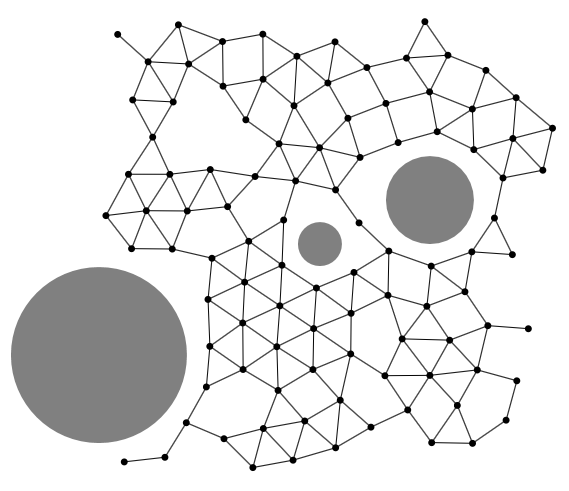
\includegraphics[width=6cm]{obstacles.png}
  \end{figure}

\end{frame}

\end{document}
